\chapter{Convolutional Neural Networks (CNN)}
\section{Tensor notation}
\begin{definition}
A tensor $T$ of order $d$  is a multi-index array,
\begin{equation}
T \in \mathbb R^{n_1 \times n_2 \times \cdots \times n_d},
\end{equation}
with $i$-th dimension being $n_i$. 
\end{definition}
\paragraph{Example 1: 2D grey image}
\begin{equation}\label{2DGreyImage}
T \in \mathbb{R}^{n_1 \times n_2}.
\end{equation}
\paragraph{Example 2: 2D color image}
\begin{equation}\label{2DColorImage}
T \in \mathbb{R}^{3 \times n_1 \times n_2}.
\end{equation}
\paragraph{Example 3: 3D grey image - MRI}
\begin{equation}\label{3DColorImage}
T \in \mathbb{R}^{ n_1 \times n_2 \times n_3}.
\end{equation}

\begin{definition}[Tensor Product]
If $X \in \mathbb R^{n_1 \times n_2 \times \cdots \times n_d}$ and $Y \in \mathbb R^{m_1 \times m_2 \times \cdots \times m_e}$, then the tensor product is noted as $\otimes$ with the next definition, 
\begin{equation}
X \otimes Y \in \mathbb R^{n_1 \times n_2 \times \cdots \times n_d \times m_1 \times m_2 \times \cdots \times m_e},
\end{equation}
with 
\begin{equation}
(X\otimes y)_{i_1, \cdots, i_d, j_1, \cdots,j_e} = X_{i_1, \cdots, i_d} Y_{j_1, \cdots, j_e}.
\end{equation}
\end{definition}
\paragraph{Example 5: Rank one matrix} If $x \in \mathbb{R}^n$ and $y \in \mathbb{R}^m$, then
\begin{equation}\label{3DColorImage}
x \otimes y \in \mathbb{R}^{n \times m},
\end{equation}
with 
\begin{equation}
x \otimes y = x y^\top.
\end{equation}

\paragraph{Example 6: } If $X \in \mathbb{R}^{n_1\times n_2}$ and $Y \in \mathbb{R}^{m_1 \times m_2}$, then
\begin{equation}\label{3DColorImage}
X \otimes Y \in \mathbb{R}^{n_1 \times n_1 \times m_1 \times m_1},
\end{equation}
with 
\begin{equation}
(X \otimes Y)_{i_1, i_2, j_1 ,j_2}  =  X_{i_1, i_2} Y_{j_1, j_2}.
\end{equation}

\begin{definition}[Tensor ``inner product"]
If 
$$
X \in \mathbb R^{(n_1 \times n_2 \times \cdots \times n_d )\times
  (t_1\times t_2\times\cdots\times t_k)}
$$ and 
$$
Y\in \mathbb R^{ (t_k\times t_{k-1}\times\cdots\times t_1)\times
  (m_1 \times m_2 \times \cdots \times m_e)},
$$
then the tensor ``inner product" with order $k$ is given by
\begin{equation}
X\odot_k Y \in \mathbb R^{n_1 \times n_2 \times \cdots \times n_d \times m_1 \times m_2 \times \cdots \times m_e},
\end{equation}
with 
\begin{equation}
(X\odot_k Y)_{i_1, \cdots, i_d, j_1, \cdots,j_e} 
=\sum_{s_1=1}^{t_1} \cdots\sum_{s_k=1}^{t_k}X_{i_1, \cdots, i_d, s_1,\cdots,s_k} Y_{s_k,\cdots,s_1,,j_1, \cdots, j_e}.
\end{equation}
\end{definition}
We note that
$$
X\otimes Y =X\odot_0Y
$$
For simplicity, we denote
\begin{equation}
X\cdot Y=X\odot_1Y \mbox{ and } X:Y=X\odot_2 Y  .
\end{equation}
\paragraph{Example 7: } If $x \in \mathbb{R}^{1\times n}$ and $y \in \mathbb{R}^{n}$, then
\begin{equation}\label{3DColorImage}
x \odot_1 y =xy= \sum_{i=1}^n x_{1,i} y_{i,1}.\in \mathbb{R}^{1}. 
\end{equation}


\paragraph{Example 8: } If $X \in \mathbb{R}^{n_1 \times m}$ and $Y \in \mathbb{R}^{m \times n_2}$, then
\begin{equation}\label{3DColorImage}
X \odot_2 Y =XY\in \mathbb{R}^{n_1 \times n_2},
\end{equation}
with 
\begin{equation}
(X \cdot Y)_{i,j} = \sum_{k=1}^m X_{i,k} Y_{k,j}.
\end{equation}
which is again the product of two matrices. 

\section{Single layer with vector space}
A singular layer linear neural network can be written as
$$
f(x, \theta)
=
\begin{pmatrix}
  f_1(x,\theta_1)\\
\vdots
\\
  f_m(x,\theta_m)
\end{pmatrix}
=
\begin{pmatrix}
 w_1 x+b_1, \\
\vdots
\\
 w_m x+b_m, \\
\end{pmatrix}
=
\begin{pmatrix}
 w_1\\
\vdots
\\
 w_m
\end{pmatrix}x
+
\begin{pmatrix}
b_1\\
\vdots
\\
b_m
\end{pmatrix}
=Wx+b=\theta \tilde x
$$
where
\begin{equation}
W\in \mathbb R^{m\times n}, 
\theta=(W,b)=
\begin{pmatrix}
  \theta_1\\
\vdots\\
\theta_m
\end{pmatrix}, \quad
\tilde x=
\begin{pmatrix}
  x\\
1
\end{pmatrix}
\end{equation}


We have
\begin{equation}
f(x; \theta )= W x+b, ~ \Theta = \{ \theta = (W,b) ~|~ W \in \mathbb{R}^{m \times n}, b \in \mathbb{R}^m \}.
\end{equation}

with $f: \mathbb{R}^n \to \mathbb{R}^m$.

\section{Deep neural networks (DNN) with vector space}
\begin{figure}[!ht]        
\center{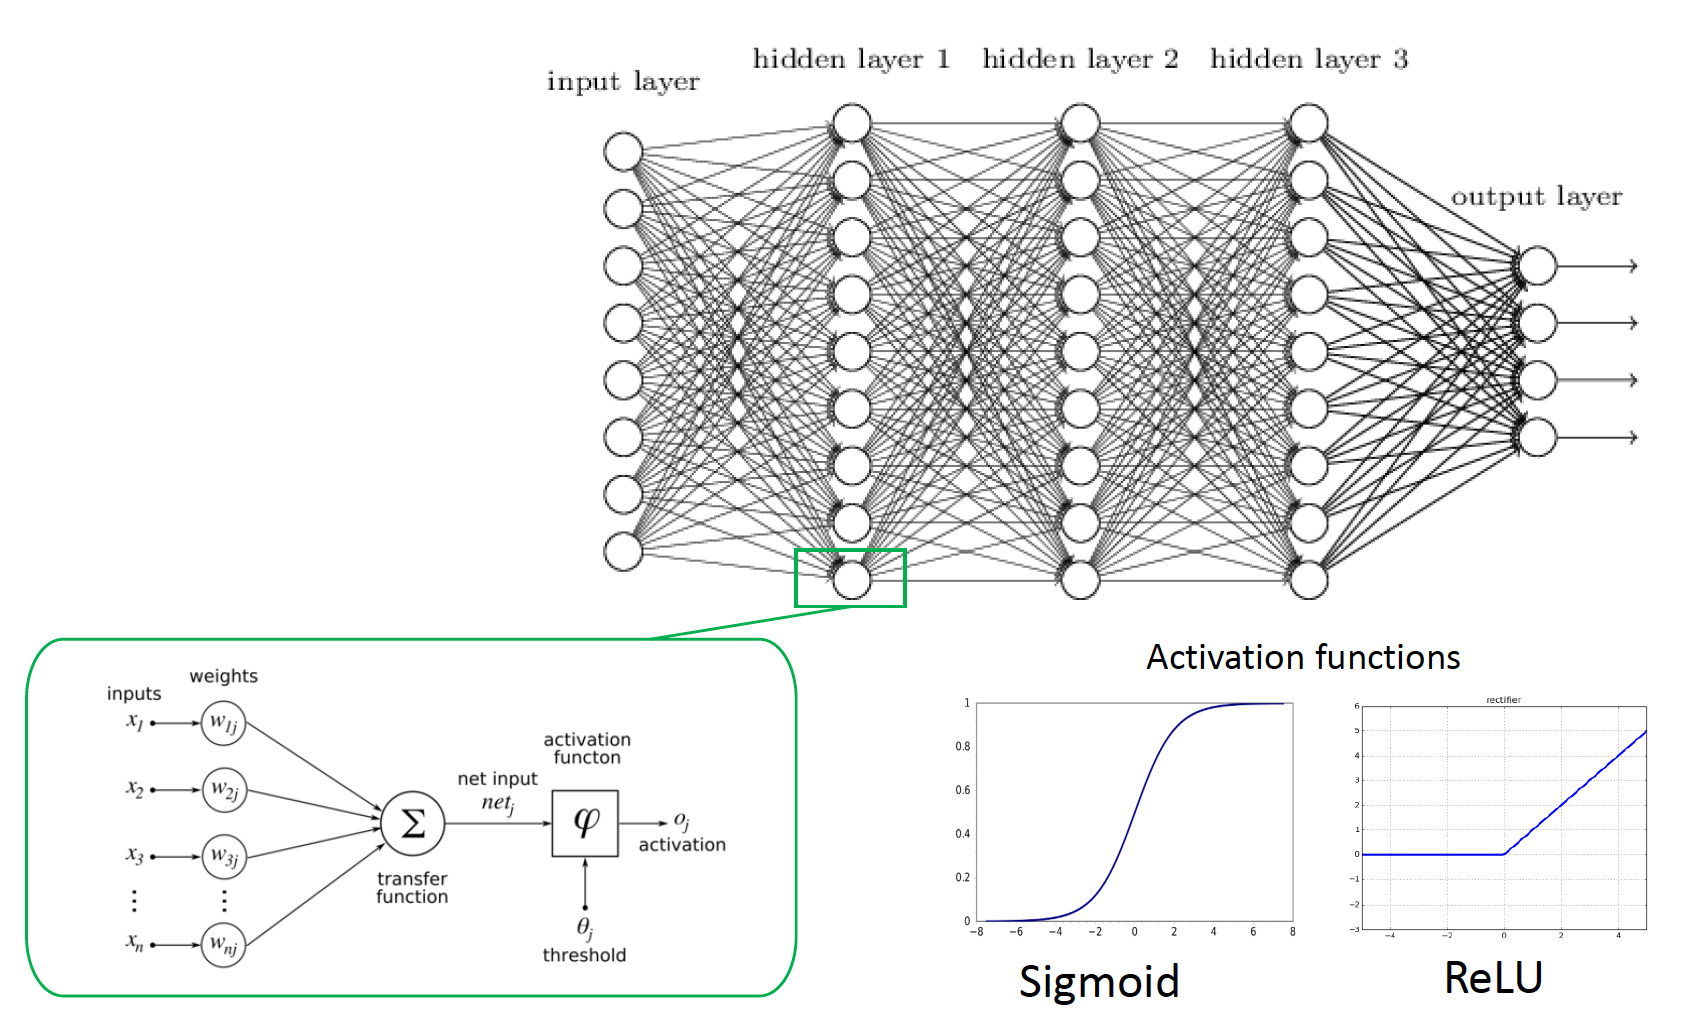
\includegraphics[width=12cm,height=6cm] {figures/ANN.png}}        
\caption{A typical deep neural network}      
\end{figure}
We consider a sequence of affine operations:
\begin{equation}
\theta^j: \mathbb R^{\hat{n}^{j}}\mapsto \mathbb R^{ n^{j}}.   
\end{equation}
with
\begin{equation}\label{DNN_affinemap}
\theta^j(x) =  W^j x + b^j 
=
(W^j, b^j) \cdot
\begin{pmatrix}
  x \\
1
\end{pmatrix}
=
\theta^j \cdot
\begin{pmatrix}
  x \\
1
\end{pmatrix}
\end{equation}
and 
\begin{equation}
W^j\in \mathbb R^{n^j \times  \hat n^{j}}, b^j\in \mathbb R^{n^j}.
\end{equation}
With a slight abuse of notation, we also denote
\begin{equation}
\theta^j=(W^j, b^j)
=
\begin{pmatrix}
\theta^j_{1}\\
\vdots \\  
\theta^j_{n^j}\\
\end{pmatrix}
\in \mathbb R^{n^j\times (\hat n^{j}+1)}.
\end{equation}

For $j=0$, we have the input data 
$$
x\in \mathbb R^{\hat n^{0}}
$$
For MNIST data base, we have
$$
\hat n^0 = 784.
$$

We consider nonlinear activation function that is applied componentwise:
\begin{equation}\label{DNN_iteration_vector}
g:\mathbb R^{ n^{j-1}}\mapsto \mathbb R^{n^{j-1}},
\end{equation}
and polling functions
\begin{equation}\label{DNN_iteration_vector}
r^j:\mathbb R^{ n^{j-1}}\mapsto \mathbb R^{\hat n^{j}}. 
\end{equation}
Poolling is not always applied after each application of activation.
When it is not applied, $r^j$ is identity and $\hat n^j=n^{j-1}$;   when
it is applied, $r_j$ is usually nonlinear and
$$
\hat n^j<n^{j-1}. 
$$

We consider the pooled-activation functions:
\begin{equation}\label{DNN_iteration_vector}
g^j=r^j\circ g: \mathbb R^{{n}_{j-1}}\mapsto
\mathbb R^{\hat n^{j}}, \quad j =  1 :J.
\end{equation}
We note that
\begin{equation}
\theta^j\circ g^j:    \mathbb R^{{n}^{j-1}}\mapsto
\mathbb R^{n^{j}}
\end{equation}

We can then define a multi-layer neural network
	\begin{equation}\label{DNN_finallayer}
	f(x; \Theta) = f^J,
	\end{equation}
        in terms of the following recursive relation:
	\begin{equation}\label{DNN_iteration_vector}
	f^j(x,\Theta^j) = (\theta^j\circ g^j\circ
        f^{j-1})(x,\Theta^{j-1}), \quad j=1:J
	\end{equation}
where
\begin{equation}
\Theta^j=(\Theta^{j-1},\theta^j), \quad \Theta^0=\theta^0
\end{equation}
and
	\begin{equation}
	f^0(x)=\theta^0(x)
	\end{equation}
	and 

\begin{align}
\Theta =\Theta_J =(\theta^0,\theta^1, \cdots, \theta^J)=( ({W^0}, {b^0}),({W^1}, {b^1}),
\cdots, ({W^J}, {b^J})) \\
\displaystyle
	\in  (\mathbb{R}^{n^0 \times (\hat n^0 + 1)}) \oplus \cdots
        \oplus  	(\mathbb{R}^{{n}_{J} \times (\hat
          n^{J}+1)})=
\oplus_{j=0}^J \mathbb{R}^{n^{j} \times (\hat n^{j} + 1)}
\end{align}


\subsection{DNN models with tensor notation}
\subsubsection{General setup}
Data:
	\begin{itemize}
		\item Input set: $\bm{X} = \{x_1, \cdots, x_N\}$
		\item Output set: $\bm{y} =  \{y_1, \cdots, y_N\}$
		\item Generally,  input use $x \in \mathbb{R}^{ n^0_1\times \cdots \times n^0_{d^0} }$, with a label $y \in \mathbb{R}^{m_1 \times \cdots \times m_c}$
		%\item Here $\hat c_0$ means the channel dimension and $\hat n_1\times \cdots \times \hat n_d$ means the essential dimension.
	\end{itemize}


Now we first construct the linear operation:
$$
\theta^j: \mathbb{R}^{ n^j_1\times \cdots \times n^j_{d^{j}} } \mapsto  \mathbb{R}^{ n^{j+1}_1\times \cdots \times n^{j+1}_{d^{j+1}} },
$$
with
\begin{equation}\label{DNN_tensor_affinemap}
\theta^j(x) =  W^j \odot_{d^j} x + b^j \in \mathbb R^{n^{j+1}_1 \times \cdots \times  n^{j+1}_{d^{j+1}}},
\end{equation}
with dimension of $W^j$ and $b^j$ as
\begin{equation}\label{space:W&b}
W^j \in \mathbb{R}^{ \left(n^{j+1}_1 \times \cdots \times n^{j+1}_{d^{j+1}}\right) \times \left(n^j_1\times \cdots \times n^j_{d^{j}}\right) }, \quad b^j \in \mathbb R^{n^{j+1}_1 \times \cdots \times  n^{j+1}_{d^{j+1}}}.
\end{equation}
Then the above equation can be expressed by a extended system like:
\begin{equation}\label{DNN:extend}
\theta^j(x) = \tilde W^j \odot_{d^j} \tilde x.
\end{equation}
Here we have the extended version of $x$ and $W$ as combine $b$ into $W$:
\begin{itemize}
	\item Extension of $x$
\begin{equation}\label{space:extend^x}
\tilde x  \in \mathbb{R}^{ (n^j_1 + 1)\times \cdots \times (n^j_{d^{j}} + 1) },
\end{equation}
with 
\begin{equation}\label{form:extend^x}
\begin{cases}
&\tilde x[1:n^j_{1},\cdots,1:n^{j}_{d^{j}}] = x, \\
 &\tilde x[(n^j_1 + 1), \cdots, (n^j_{d^{j}} + 1) ] = 1, \\
 &\tilde x[i_1,\cdots,i_{d^j}] = 0 \quad \text{others}.
\end{cases}
\end{equation}
	\item Extension of $W^j$
\begin{equation}\label{space:extend^W}
\tilde W^j  \in \mathbb{R}^{ \left(n^{j+1}_1 \times \cdots \times n^{j+1}_{d^{j+1}}\right) \times \left((n^j_1 + 1)\times \cdots \times (n^j_{d^{j}} + 1)\right) },
\end{equation}
with 
\begin{equation}\label{form:extend^W}
\begin{cases}
&\tilde W^j[1:n^{j+1}_1,\cdots,1:n^{j+1}_{d^{j+1}},1:n^j_{1},\cdots,1:n^{j}_{d^{j}}] = W, \\
&\tilde W^j[1:n^{j+1}_1,\cdots,1:n^{j+1}_{d^{j+1}},(n^j_1 + 1), \cdots, (n^j_{d^{j}} + 1) ] = b^j, \\
&\tilde W^j[i_1,\cdots,i_{d^j},j_1,\cdots,] = 0 \quad \text{others}.
\end{cases}
\end{equation}
\end{itemize}

\subsubsection{Example of extended form of affine map for 1st and 2nd order tensor}
\begin{itemize}
	\item For 1st order tensor(vector space) \\
	For this cases, $d^j = 1$ for all $j$ or we can have:
	\begin{equation}
	x \in \mathbb{R}^{n}, \quad W \in \mathbb{R}^{m \times n}.
	\end{equation}
	Then we have the extended form as:
	\begin{equation}\label{extend:1st}
	\tilde x = \begin{pmatrix}
	x \\
	1
	\end{pmatrix}, \quad \tilde W = (W, b),
	\end{equation}
	for $b \in \mathbb{R}^m$.
	\item Convolution model for image without channels(2nd order tensor) \\
	For this case, $d_j = 2$ for all $j$ or we can have:
	\begin{equation}
	x \in \mathbb{R}^{n_1 \times n_2}, \quad W \in \mathbb{R}^{(m_1\times m_2) \times (n_1\times n_2)}.
	\end{equation}
	Then we have the extended form for $x$:
	\begin{equation}\label{extend:2nd_x}
	\tilde x = \begin{pmatrix}
	x & 0\\
	0 & 1
	\end{pmatrix}.
	\end{equation}
	For $W$, because it is a 4th order tensor, we cannot express it as a matrix form, we can only have
	\begin{equation}\label{extend:2nd_W}
	\begin{cases}
	&\tilde W[1:m_1, 1:m_2,1:n_{1},1:n_{2}] = W, \\
	&\tilde W[1:m_1,1:m_{2},(n_1 + 1), (n_{2} + 1) ] = b, \\
	&\tilde W[1:m_1,1:m_{2},1:n_1, (n_{2} + 1)] = 0 \\
	&\tilde W[1:m_1,1:m_{2}, (n_1+1), 1:n_{2}] = 0.
	\end{cases}
	\end{equation}
\end{itemize}


\subsection{BP Algorithm:}

Under the above notation and iteration structure, we have:
\begin{equation}\label{BP_recursion}
\frac{\partial f^j}{\partial \theta^i} = \begin{cases}
0 \quad &\text{if} \quad i > j, \\
I_{n_j} \otimes \begin{pmatrix}
g^{j}(f^{j-1}) \\
1 
\end{pmatrix} \quad &\text{if} \quad i = j,\\
W^j  \frac{\partial g^{j}(f^{j-1})}{\partial f^{j-1}} \cdot \frac{\partial f^{j-1}}{\partial \theta^i}  \quad &\text{if} \quad i < j.
\end{cases}
\end{equation}
So, the BP algorithm is to use the \eqref{BP_recursion} to compute
\begin{equation}
\frac{\partial f^J}{\partial {\Theta} } 
= \left\{
\frac{\partial  f^J}{\partial {\theta^0} }, 
\frac{\partial  f^J}{\partial {\theta^1} }, 
\cdots \frac{\partial f^J}{\partial
	{\theta^J} }\right\} \in {\rm cell}
\left(
\mathbb R^{c\times n_0 \times (\hat n_0 + 1)},  
\mathbb R^{c\times n_1 \times (\hat n_1 + 1)},  
\cdots, \mathbb
R^{c\times n_{J} \times (\hat n_{J-1}+1)}
\right)
\end{equation}

Here we can check the formula \eqref{BP_recursion}:
\begin{itemize} 
	\item First for $i = j$:
	\begin{equation}
	\frac{\partial f^j_k}{\partial \theta^j_{l,s}} =
	\frac{\partial}{\partial \theta^j_{l,s}}
	\left( 
	\theta^j_{k}
	\begin{pmatrix}
	g^{j}(f^{j-1})) \\ 1 
	\end{pmatrix}
	\right) 
	= \delta_{k,l} 
	\begin{pmatrix} 
	g^{j}(f^{j-1}) \\ 1 
	\end{pmatrix}_{s}
	\end{equation}
	
	This means that:
	\begin{equation}
	\left(\frac{\partial {f^j}}{\partial {\theta^j}}\right)_{k,l,s} = \frac{\partial f^j_k}{\partial \theta^j_{l,s}} 
	= \delta_{k,l} \begin{pmatrix} g^{j}(f^{j-1}) \\ 1 \end{pmatrix}_{s} = (I_{n_j} \otimes \begin{pmatrix}
	g^{j}(f^{j-1}) \\
	1 
	\end{pmatrix})_{k,l,s}.
	\end{equation}
	
	\item Then for $i < j$; 
	\begin{equation}
	\frac{\partial f^j}{\partial \theta^i}  
	=  \frac{\partial (\theta^{j}\circ g^j)}{\partial f^{j-1}} \cdot \frac{\partial f^{j-1}}{\partial \theta^i}.
	\end{equation}
	We can check it by:
	\begin{align}
		\left(\frac{\partial f^j}{\partial \theta^i} \right)_{k,s,t} 
		= \frac{\partial f^j_k}{\partial \theta^i_{s,t}} &=
		\sum_{l = 1}^{n_{j-1}} \frac{\partial f^{j}_k}{\partial f^{j-1}_l} \frac{\partial f^{j-1}_l}{\partial \theta^i_{s,t}}  =
		\sum_{l = 1}^{n_{j-1}} \left( \frac{\partial (\theta^{j}\circ
			g^j)}{\partial f^{j-1}}\right)_{k,l} \left(\frac{\partial
			f^{j-1}}{\partial \theta^i}\right)_{l,s,t} \\  &=  
		\left(\frac{\partial  (\theta^{j}\circ g^j)}{\partial f^{j-1}} \cdot \frac{\partial f^{j-1}}{\partial \theta^i} \right)_{k,s,t}.
	\end{align}
	So what we only need to do is to compute:
	\begin{equation}
	\frac{\partial f^{j}_k}{\partial f^{j-1}_l} =\frac{ \partial}{\partial f^{j-1}_l}\left( W^j_{k} g^{j}(f^{j-1}) \right) = W^j_{k} \frac{ \partial }{\partial f^{j-1}_l}\left(g^{j}(f^{j-1})\right),
	\end{equation}
	this means that 
	\begin{equation}
	\left(\frac{\partial  (\theta^{j}\circ g^j)}{\partial
		f^{j-1}}\right)_{k,l} 
	= \frac{\partial  (\theta^{j}\circ g^j)_k}{\partial f^{j-1}_l}  = W^j_{k} \frac{ \partial}{\partial f^{j-1}_l} \left( g^{j}(f^{j-1})\right)= \left(W^j \frac{\partial }{\partial f^{j-1}}\left(g^{j}(f^{j-1})\right)\right)_{k,l}
	\end{equation}
\end{itemize}

\subsection{Classification properties under this notation}
\begin{theorem}
	If $\{A_k\}_{k=1}^c$ are separable with positive distance, then it
	can be separated by $f(x; \Theta) = f^2$, with $W^2= id, b^2=0$ and
	all activation function is $\tau$.
\end{theorem}

\section{CNN based on the DNN notation}
\subsection{General setup}
\begin{enumerate}
	\item Data:
	\begin{itemize}
		\item Input set: $\bm{X} = \{x_1, \cdots, x_N\}$
		\item Output set: $\bm{y} =  \{y_1, \cdots, y_N\}$
		\item Generally,  input use $x \in \mathbb{R}^{\hat c_0 \times \hat n_0\times \cdots \times \hat n_0 }$, with a label $y \in \mathbb{R}^c$ (output for classification problem)
		\item Here $\hat c_0$ means the channel dimension and $\hat n_1\times \cdots \times \hat n_d$ means the essential dimension.
	\end{itemize}
	\item Here we use $x \in \mathbb{R}^{\hat c_0 \times n \times n} $,
	$y \in \mathbb{R}^c$ as example.
	\item Kernels: in CNN they generally use $K^i$ and $b^i$ to stand for the kernels and bias.  
\end{enumerate}

\paragraph{Example 1: 2D grey image}
\begin{equation}\label{2DGreyImage}
c_0=1, d=2  
\end{equation}
\paragraph{Example 2: 2D color image}
\begin{equation}\label{2DColorImage}
c_0=3, d=2  
\end{equation}
\paragraph{Example 3: 3D grey image - MRI}
%\paragraph{Example 4: 3D color image?}


\subsection{A simple example of DNN for images}

Multilayer structures in convolutional layers is totally the same for \eqref{DNN_affinemap} - \eqref{DNN_finallayer}: the only difference  is the structure of affine map:

\begin{equation}\label{CNN_affinemap}
\theta^j_{p}(x) =  W^j_p \odot_3 x + b^j_p \in \mathbb R^{n_j \times n_j}, \quad p=1:c_j
\end{equation}

\begin{equation}\label{CNN_affinemap}
\theta^j(x) =  W^j\odot_3 x + b^j
\end{equation}
with 
\begin{equation}
\theta^j: \mathbb R^{\hat c_j  \times \hat{n}_{j} \times \hat n_{j} } \mapsto \mathbb{R}^{c_j \times n_{j} \times n_j }.
\end{equation}
\begin{remark}
	For many case, 
	\begin{equation}
	c_j = 2 \hat c_j,
	\end{equation}
	especially for $r^{j-1}$ is a real pooling function. 
\end{remark}
Here
\begin{equation}
W^j \in \mathbb{R}^{(c_j \times n_{j} \times n_j) \times
	(\hat{n}_{j} \times \hat n_{j}\times \hat c_{j} )}, \quad
b^j\in  \mathbb R^{c_j \times n_{j} \times n_j},  
\end{equation}
and 
\begin{align}
\theta^j  &= \{W^j , b^j\}  \in \mathbb{R}^{(c_j \times n_{j} \times n_j) \times
	(\hat{n}_{j} \times \hat n_{j}\times \hat c_{j} )} \oplus \mathbb R^{c_j \times n_{j} \times n_j} \\ 
&\cong  \mathbb{R}^{(c_j \times n_{j} \times n_j) \times
	(\hat{n}_{j} \times \hat n_{j}\times c_{j} + 1 )}
\end{align}

We note that
\begin{equation}
\hat n_0 =n  
\end{equation}

We consider nonlinear activation function applied element wise:
\begin{equation}\label{CNN_iteration_vector}
g: \mathbb R^{c_{j-1} \times n_{j-1} \times n_{j-1} }\mapsto  \mathbb R^{c_{j-1} \times n_{j-1} \times n_{j-1}},
\end{equation}
and polling functions
\begin{equation}\label{CNN_iteration_vector}
r^j: \mathbb R^{c_{j-1} \times n_{j-1} \times n_{j-1} }\mapsto  \mathbb R^{\hat c_j \times \hat n_{j} \times\hat n_j }. 
\end{equation}

We consider ``pooled-activation'' functions:
\begin{equation}\label{CNN_iteration_vector}
g^j=r^j\circ g:  \mathbb R^{c_{j-1} \times n_{j-1} \times n_{j-1} }\mapsto
\mathbb  \mathbb R^{\hat c_j \times \hat n_{j} \times \hat n_j }, \quad j  = 1:J. 
\end{equation}
\begin{remark}
	Generally speaking, we have 
	\begin{equation}
	\hat c_{j} = c_{j-1},
	\end{equation}
	for almost cases.
	
	But, some times, when the channel size is big enough,  they would like to take:
	\begin{equation}
	\hat c_{j} = \frac{c_{j-1}}{2}.
	\end{equation}
	to reduce the channel dimension by adding two channels as one then using $r$ or just using the max-pooling for both this two channel and get one out put.
	
\end{remark}


We have the multi-layer DNN structure like:
\begin{equation}\label{CNN_iteration_vector}
f^j(x,\Theta^j) = (\theta^j\circ g^{j}\circ f^{j-1})(x,\Theta^{j-1}) \in \mathbb{R}^{c_j \times n_j \times n_j }
\end{equation}
where
\begin{equation}
\Theta^j=(\Theta^{j-1},\theta^j), \quad \Theta^0=\theta^0 
\end{equation}
with 
\begin{equation}
f^0(x)=\theta^0(x)
\end{equation}
and 
\begin{equation}\label{CNN_finallayer}
f(x; \Theta) = f^J.
\end{equation}

Roughly speaking, \eqref{CNN_affinemap} -
\eqref{CNN_finallayer} a special case of \eqref{DNN_affinemap}
- \eqref{DNN_finallayer} in tensor notation.


\subsection{Convolution structure for images}
A convolution operation is a special linear mapping of the following form:
\begin{equation}
\theta^j(x) = K^j \circledast x + {\rm{diag}(b^j)} \cdot \bm{1}_{c_j \times n_j \times n_j} \quad
\in\mathbb R^{c_j\times n_j\times n_j}.
\end{equation}
with 
\begin{equation}
K^j \in \mathbb{R}^{ c_{j} \times \hat c_{j} \times (2k+1) \times (2k+1)},  \quad \text{and} \quad b^j \in \mathbb{R}^{c_j},
\end{equation}
and 
\begin{equation}
\bm{1}_{c_j \times n_j \times n_j} = 1_{c_{j}} \otimes 1_{n_j} \otimes 1_{n_j}
\end{equation}
for $k = 0, 1, 2, 3...$.

Give $p\in \{1,\ldots c_j\}$
\begin{equation}
(\theta^j(x))_p= (K^j \circledast x)_p+b^j_p{\bm 1}_{n_j\times n_j}
\end{equation}
and
\begin{equation}
(K^j \circledast x)_p
= \sum_{q=1}^{\hat c_{j}} K^{j}_{p,q} \ast x_q \in \mathbb{R}^{n_j \times n_j}, \quad p= 1:c_j.
\end{equation}
where
$$
K^{j}_{p,q}\in \mathbb R^{(2k+1)\times (2k+1)}, x_q\in \mathbb
R^{\hat n_{j}\times \hat n_{j}}.
$$
Here $\ast$ is the traditional convolution defined as:
\begin{equation}\label{ConvPadding}
(K \ast x)_{i,j} :=\sum_{s, t = -k}^k  K_{s+k+1,t+k+1} x_{i + s, j + t},
\end{equation}
Here we assume implicitly that a special ``padding'' is used such that
\begin{equation}
\label{zero-padding}
x_{i,j}=0 \mbox{ if } i, j\le 0 \mbox{ or } i, j > n_j.  
\end{equation}

\bigskip \hrule \bigskip  
\begin{example} ~
\begin{enumerate}
	\item 
	For $j=1$, $c_0=3, \hat n_0=n$.   We can take $c_1$ different channels
	\begin{equation}
	(K^1 \circledast x)_p= \sum_{q=1}^{\hat{c}_1=3} K^{j}_{p,q} \ast x_q \in \mathbb{R}^{n_j \times n_j}, \quad p= 1:c_1.
	\end{equation}
	\item We take $c_2$ different channels
	\begin{equation}
	\left(\theta^2(K^1 \circledast x)\right)_p= \sum_{q=1}^{\hat c_2} K^{j}_{p,q} \ast g^2\left((K^1 \circledast x)_q\right) + b^2_p{\bm 1}_{n_2\times n_2} \in \mathbb{R}^{n_j \times n_j}, \quad p= 1:c_2.
	\end{equation}
\end{enumerate}
\end{example}
\bigskip \hrule \bigskip  


\begin{remark}
	We recall the standard definition of convolution of two tensor:
	\begin{equation}
	\label{standard-convolution}
	(u\ast x)_{i,j}=\sum_{k,\ell=-\infty}^\infty u_{i-k,j-\ell}x_{k,\ell}  
	\end{equation}
	The definitions of \eqref{ConvPadding} and
	\eqref{standard-convolution} are related by taking $u$ to be a ``locally
	supported'' tensor and using appropriate paddings.
\end{remark}


So, we say that CNN is a special cases means the above process has those next properties:
\begin{properties} Under the notation  \eqref{CNN_affinemap} - \eqref{CNN_finallayer}:
	\begin{enumerate}
		\item $\hat n_{j} = n_j$. Or some times they do convolutions without padding such that $\hat n_{j} = n_j + 2k$, with kernel size $2k+1$.
		
		\item $n_{j-1} = 2 \hat n_j$ in some cases. 
		\item Choice of pooling function:
		\begin{equation}
		\label{pooling}
		r(x)=R\ast x+rn(x)
		\end{equation}
		where 
		\begin{equation}
		[n(x)]_{i,j}=\| (x_{2i+k,2j+l}: k,l=-1,0,1)\|, \quad i,j=1:\hat n_j
		\end{equation}
		where $\|\cdot\|$ is either $\ell^p$-norm for $p=2$ or $\infty$. 
	\end{enumerate}
	or 
	\begin{equation}
	\label{pooling2}
	r(x)=R\ast x+r_2 n_2(x)+r_\infty n_\infty(x)
	\end{equation}
	where $n_p(x)$ corresponds to local $\ell^p$ norm.
\end{properties}
For $p=\infty$, we may not take the actual $\ell^\infty$ norm, but
rather take the maximum without taking absolute value:
$$
[n_\infty(x)]_{ij}=\max_{-1\le k,l\le 1} x_{2i+k, 2j+l}
$$

For example, 
\begin{equation}
\label{stride-pooling}
[r(x)]_{ij}=R\ast x_{2i,2j}+rn(x)_{2i,2j}, i, j=1:\hat n_{\ell}
\end{equation}
If we take $r=0$,  the above procedure is precisely what is so-called
``stride'' in the literature.   This means that, the stride is just a
special pooling that defines a ``coarse'' point as a linear
combination of its neighbors and the underlying coefficients will be
obtained from the training process. 

\subsection{Understand channel as multi-coarse space}
We want to under stand the channels in CNN by the multi-coarse space in AMG. The idea is that, if we have $c$ channels as the input, we want to get some multi-coarse space with or just do some smoother in this level.

\subsection{Convolution with stride for image}
Stride is a very convenient way(maybe the simplest way) to reduce the essential dimension of images. And it can be combined with classical convolution very easily as there are both linear operation.
\subsubsection{Definition of stride}
If we use stride $s$, we have have the stander convolution operator with stride $s$ as:
\begin{equation}\label{equ:convstride}
(K\ast_{s} x)_{i,j} = \sum_{p, q = -k}^k K_{p+k+1,q+k+1}x_{is + p, js + q} .
\end{equation}
This stride properties in some application are often used as pooling(subsampling, coarsening).  

Here we can define a special pooling operator as $S(\cdot,s)$ which likes the $C/F$ split for choosing coarse point:
\begin{equation}
S(X,s)_{i,j} = X_{is, js },
\end{equation}
then we have:
\begin{equation}\label{equ:stride}
X \ast_s K = S(X\ast K, s),
\end{equation}
with the $\ast$ and $\ast_s$ defined by \eqref{ConvPadding} and \eqref{equ:convstride}
\begin{proof}
	\begin{align}
	S(X \ast K,s)_{i,j} &= (X \ast K)_{is, js}  \\
	&= \sum_{p, q = -k}^k K_{p+k+1,q+k+1}x_{is + p, js + q}  \\
	&= (X \ast_s K)_{i,j}.
	\end{align}
\end{proof}

\begin{remark}
	Here we need to mark that, in fact, the stride operation is just a kind of special coarse operations. The convolution with stride is in fact a kind of restriction operation with certain coarse strategy and some trained restrictions operations. 
\end{remark}



\subsubsection{Add stride without change $\theta^j$}
\begin{enumerate}
	
	\item Convolution: 
	\begin{equation}
	\theta^j: \mathbb R^{\hat c_j \times \hat{n}_{j} \times \hat n_{j} } \mapsto \mathbb{R}^{c_j \times n_{j} \times n_j }.
	\end{equation}
	with
	\begin{equation}
	\theta^j(x) = K^j \circledast x + {\rm{diag}(b^j)} \cdot \bm{1}_{c_j \times n_j \times n_j} \quad
	\in\mathbb R^{c_j\times n_j\times n_j}.
	\end{equation}
	with 
	\begin{equation}
	K^j \in \mathbb{R}^{ c_{j} \times \hat c_{j} \times (2k+1) \times (2k+1)},  \quad \text{and} \quad b^j \in \mathbb{R}^{c_j},
	\end{equation}
	and 
	\begin{equation}
	\bm{1}_{c_j \times n_j \times n_j} = 1_{c_{j}} \otimes 1_{n_j} \otimes 1_{n_j}
	\end{equation}
	for $k = 0, 1, 2, 3...$.
	
	\item Stride: 
	\begin{equation}
	S^{j-1}: \mathbb R^{ c_{j-1} \times {n}_{j-1} \times  n_{j-1}} \mapsto \mathbb{R}^{ c_{j-1} \times\tilde n_{j-1} \times\tilde  n_{j-1} }.
	\end{equation}
	with
	\begin{equation}
	S^{j-1}(X) = S(X, s^{j-1}),
	\end{equation}
	for $s^{j-1} = 1$ for almost $j$ and $s^{j-1} = 2$ for near $\log \hat n_0$ times.
	
	\item Activation: 
	\begin{equation}\label{CNN_iteration_vector}
	g: \mathbb R^{c_{j-1} \times \tilde n_{j-1} \times \tilde  n_{j-1} }\mapsto  \mathbb R^{c_{j-1} \times \tilde n_{j-1} \times \tilde n_{j-1}},
	\end{equation}
	
	\item Polling:
	\begin{equation}\label{CNN_iteration_vector}
	r^j: \mathbb R^{c_{j-1} \times \tilde n_{j-1} \times\tilde n_{j-1} }\mapsto  \mathbb R^{\hat c_j \times \hat n_{j} \times\hat n_j }. 
	\end{equation}
\end{enumerate}


So we have the stander CNN model with stride as:
\begin{itemize}
	\item {\color{red} $S^j \circ \theta^j\circ r^j\circ g$ form:}
	\bigskip \hrule \bigskip  
	\begin{equation}\label{CNN_stride_iteration_vector}
	f^j(x,\Theta^j) = (S^j \circ \theta^j\circ r^j\circ g\circ f^{j-1})(x,\Theta^{j-1}) \in \mathbb{R}^{c_j \times \tilde n_j \times \tilde n_j }
	\end{equation}
	where
	\begin{equation}
	\Theta^j=(\Theta^{j-1},\theta^j), \quad \Theta^0=\theta^0 
	\end{equation}
	with 
	\begin{equation}
	{\color{red} f^0(x)=S^0 \circ \theta^0(x)}
	\end{equation}
	and 
	\begin{equation}\label{CNN_finallayer}
	f(x; \Theta) = f^J.
	\end{equation}
	\bigskip \hrule \bigskip  
	
	\item {\color{red} $\theta^j\circ r^j\circ g \circ S^{j-1} $ form:}
	\bigskip \hrule \bigskip  
	\begin{equation}\label{CNN_stride_iteration_vector}
	f^j(x,\Theta^j) = (\theta^j\circ r^j\circ g \circ S^{j-1} \circ f^{j-1})(x,\Theta^{j-1}) \in \mathbb{R}^{c_j \times n_j \times n_j }
	\end{equation}
	where
	\begin{equation}
	\Theta^j=(\Theta^{j-1},\theta^j), \quad \Theta^0=\theta^0 
	\end{equation}
	with 
	\begin{equation}
	{\color{red} f^0(x)=\theta^0(x)}
	\end{equation}
	and 
	\begin{equation}\label{CNN_finallayer}
	f(x; \Theta) = f^J.
	\end{equation}
	\bigskip \hrule \bigskip  
\end{itemize}

We can use those next plans for simplify \eqref{CNN_stride_iteration_vector}. 
\begin{enumerate}
	\item {\color{red} For $S^j \circ \theta^j\circ r^j\circ g$ form,} we can note stride with convolution together:
	\bigskip \hrule \bigskip 
	We can consider ``stride-convolution'' functions:
	\begin{equation}\label{CNN_iteration_vector}
	C^j =S^j\circ \theta^j:  \mathbb R^{\hat c_{j} \times\hat n_{j} \times\hat n_{j} }\mapsto
	\mathbb  \mathbb R^{c_j \times \tilde n_{j} \times \tilde n_j }, \quad j  = 1:J. 
	\end{equation}
	
	Then we consider ``pooled-activation'' functions:
	\begin{equation}\label{CNN_iteration_vector}
	g^j=r^j\circ g:  \mathbb R^{c_{j-1} \times n_{j-1} \times n_{j-1} }\mapsto
	\mathbb  \mathbb R^{\hat c_j \times \hat n_{j} \times \hat n_j }, \quad j  = 1:J. 
	\end{equation}
	
	At last get \eqref{CNN_stride_iteration_vector} as:
	\begin{equation}\label{CNN_stride_iteration_vector_1}
	f^j(x,\Theta^j) = (C^j \circ g^j\circ f^{j-1})(x,\Theta^{j-1}) \in \mathbb{R}^{c_j \times n_j \times n_j }
	\end{equation}
	
	
	\bigskip \hrule \bigskip  
	
	\item {\color{red} For $S^j \circ \theta^j\circ r^j\circ g$ form,} we can note stride, convolution and pooling together:
	
	\bigskip \hrule \bigskip  
	We consider ``stride-convolution-pooling'' functions:
	\begin{equation}\label{CNN_iteration_vector}
	\theta^j=S^j\circ \theta^j \circ r^j:  \mathbb R^{c_{j-1} \times \tilde n_{j-1} \times\tilde n_{j-1} }\mapsto
	\mathbb  \mathbb R^{c_j \times \tilde n_{j} \times \tilde n_j }, \quad j  = 1:J. 
	\end{equation}
	
	At last get \eqref{CNN_stride_iteration_vector} as:
	\begin{equation}\label{CNN_stride_iteration_vector_2}
	f^j(x,\Theta^j) = (\theta^j \circ g\circ f^{j-1})(x,\Theta^{j-1}) \in \mathbb{R}^{c_j \times n_j \times n_j }
	\end{equation}
	\bigskip \hrule \bigskip  
	
	
	
	\item {\color{red} For $\theta^j\circ r^j\circ g \circ S^{j-1} $ form:} We can note stride with nonlinear layer together:
	\bigskip \hrule \bigskip  
	We consider ``stride-pooled-activation'' functions:
	\begin{equation}\label{CNN_iteration_vector}
	g^j=r^j\circ g \circ S^{j-1}:  \mathbb R^{c_{j-1} \times n_{j-1} \times n_{j-1} }\mapsto
	\mathbb  \mathbb R^{\hat c_j \times \hat n_{j} \times \hat n_j }, \quad j  = 1:J. 
	\end{equation}
	
	At last get \eqref{CNN_stride_iteration_vector} as:
	\begin{equation}\label{CNN_stride_iteration_vector_2}
	f^j(x,\Theta^j) = (\theta^j \circ g^j\circ f^{j-1})(x,\Theta^{j-1}) \in \mathbb{R}^{c_j \times n_j \times n_j }
	\end{equation}
	\bigskip \hrule \bigskip  
	
\end{enumerate}

\subsubsection{Merge stride into $\theta^j$}
Besides this,  we can merge stride into convolution as:
\begin{equation}
\theta^j: \mathbb R^{\hat c_j \times \hat{n}_{j} \times \hat n_{j} } \mapsto \mathbb{R}^{c_j \times n_{j} \times n_j }.
\end{equation}
with
\begin{equation}
\theta^j(x) = K^j \circledast_{s^j} x + {\rm{diag}(b^j)} \cdot \bm{1}_{c_j \times n_j \times n_j} \quad
\in\mathbb R^{c_j\times n_j\times n_j}.
\end{equation}
with 
\begin{equation}
K^j \in \mathbb{R}^{ c_{j} \times \hat c_{j} \times (2k+1) \times (2k+1)},  \quad \text{and} \quad b^j \in \mathbb{R}^{c_j},
\end{equation}
and 
\begin{equation}
\bm{1}_{c_j \times n_j \times n_j} = 1_{c_{j}} \otimes 1_{n_j} \otimes 1_{n_j}
\end{equation}
for $k = 0, 1, 2, 3...$.

Give $p\in \{1,\ldots c_j\}$
\begin{equation}
(\theta^j(x))_p= (K^j \circledast_{s^j} x)_p+b^j_p{\bm 1}_{n_j\times n_j}
\end{equation}
and
\begin{equation}
(K^j \circledast_{s^j} x)_p
= \sum_{q=1}^{\hat c_{j}} K^{j}_{p,q} \ast_{s^j} x_q \in \mathbb{R}^{n_j \times n_j}, \quad p= 1:c_j.
\end{equation}
where
$$
K^{j}_{p,q}\in \mathbb R^{(2k+1)\times (2k+1)}, x_q\in \mathbb
R^{\hat n_{j}\times \hat n_{j}}.
$$
Here $\ast_{s^j}$ is the stander convolution with stride as definition before.


At last, we keep \eqref{CNN_stride_iteration_vector} unchanged. What's more, we can have the next relation:
\begin{equation}
n_j = \frac{\hat n_j}{s^j}.
\end{equation}
 



\newpage
\subsection{Restriction: a combination of pooling and stride}
Here we consider as our restriction function as:
\begin{equation}
r(x) = sC(x) + nN(x),
\end{equation}
with combination parameters $s, n \in \mathbb R$, and $N(x)$ is the traditional pooling function like $\ell^{p}$ normal with $p = 1$ or $p = \infty$. However, we define $C(x)$ as an extension version of traditional ``convolution with stride" operation like:
\begin{equation}
(C(x))_{i,j} = \sum_{s,t = -k}^{k}K_{i,j,s,t}x_{pi + s, pj + t}.
\end{equation}
Or we may have this version for multi-channel:
\begin{equation}
(C(x))_{l,i,j} = \sum_{m=1}^c\sum_{s,t = -k}^{k}K_{l,m,i,j,s,t}x_{m,pi + s, pj + t}.
\end{equation}
So we will have that:
\begin{equation}
C(x) = X \ast_p K = S(X\ast K, p),
\end{equation}
if we take 
\begin{equation}
K_{i,j} = K_{\tilde i, \tilde j} \in \mathbb R^{(2k+1) \times (2k+1)}\quad  \forall i, j, \tilde i, \tilde j,
\end{equation}
or 
\begin{equation}
K_{l,m,i,j} = K_{l,m,\tilde i, \tilde j} \in \mathbb R^{(2k+1) \times (2k+1)}\quad  \forall i, j, \tilde i, \tilde j.
\end{equation}

This means that $r(x)$ can totally cover the traditional ``convolution with stride" operation, so we can have the next network structure:

\begin{enumerate}
	
	\item Convolution: 
	\begin{equation}
	\theta^j: \mathbb R^{\hat c_j \times \hat{n}_{j} \times \hat n_{j} } \mapsto \mathbb{R}^{c_j \times n_{j} \times n_j }.
	\end{equation}
	with
	\begin{equation}
	\theta^j(x) = K^j \circledast x + {\rm{diag}(b^j)} \cdot \bm{1}_{c_j \times n_j \times n_j} \quad
	\in\mathbb R^{c_j\times n_j\times n_j}.
	\end{equation}
	with 
	\begin{equation}
	K^j \in \mathbb{R}^{ c_{j} \times \hat c_{j} \times (2k+1) \times (2k+1)},  \quad \text{and} \quad b^j \in \mathbb{R}^{c_j},
	\end{equation}
	and 
	\begin{equation}
	\bm{1}_{c_j \times n_j \times n_j} = 1_{c_{j}} \otimes 1_{n_j} \otimes 1_{n_j}
	\end{equation}
	for $k = 0, 1, 2, 3...$.
	
	\item Activation: 
	\begin{equation}\label{CNN_iteration_vector}
	g: \mathbb R^{c_{j-1} \times  n_{j-1} \times   n_{j-1} }\mapsto  \mathbb R^{c_{j-1} \times n_{j-1} \times n_{j-1}},
	\end{equation}
	
	
	\item Restriction: 
	\begin{equation}
	r^j: \mathbb R^{c_{j-1} \times n_{j-1} \times n_{j-1} }\mapsto  \mathbb R^{\hat c_j \times \hat n_{j} \times\hat n_j }.\end{equation}
	with
	\begin{equation}
	r^j(x) = s^j C^j(x) + n^j N^j(x).
	\end{equation}
	
\end{enumerate}

We consider ``restriction-activation'' functions:
\begin{equation}\label{CNN_iteration_vector}
g^j=r^j\circ g:  \mathbb R^{c_{j-1} \times n_{j-1} \times n_{j-1} }\mapsto
\mathbb  \mathbb R^{\hat c_j \times \hat n_{j} \times \hat n_j }, \quad j  = 1:J. 
\end{equation}

So we have the CNN model  as:
\begin{equation}\label{CNN_iteration_vector}
f^j(x,\Theta^j) = (\theta^j\circ g^{j}\circ f^{j-1})(x,\Theta^{j-1}) \in \mathbb{R}^{c_j \times n_j \times n_j }
\end{equation}
where
\begin{equation}
\Theta^j=(\Theta^{j-1},\theta^j), \quad \Theta^0=\theta^0 
\end{equation}
with 
\begin{equation}
f^0(x)=\theta^0(x)
\end{equation}
and 
\begin{equation}\label{CNN_finallayer}
f(x; \Theta) = f^J.
\end{equation}

So we can have the next observation: 
\begin{enumerate}
	\item We can totally recover the traditional CNN model with just general pooling by 
	\begin{equation}
	s^j = 0 \quad \forall j = 1:J.
	\end{equation}
	
	\item We can also totally recover the traditional CNN model with stride $p$ by
	\begin{equation}
	n^j = 0 \quad \forall j = 1:J,
	\end{equation}
	and 
	\begin{equation}
	\theta^j = id,
	\end{equation}
	if $C^j$ works as an restriction really.
	
	\item If we keep $s^j$ and $n^j$ as two parameters to learn, we believe that this will be better than cases. 
\end{enumerate}
Let us consider a special case:
\begin{equation}
f^4=\theta^4\circ g^4\circ\theta^3\circ g^3\circ \theta^2\circ g^2\circ\theta^1\circ g^1\circ\theta_0(x)  
\end{equation}
We can regroup the different operations in different way.
\begin{equation}
f^4=\theta^4\circ r^4\circ g\circ\theta^3\circ r^3\circ g\circ
\theta^2\circ r^2\circ g\circ\theta^1\circ r^1\circ g\circ\theta_0(x)
\end{equation}

Special case 1: assuming $r^k$ represents pure stride 
\begin{equation}
f^4=\theta^4\circ g\circ r^3\circ g
\circ r^2\circ g\circ r^1\circ g\circ\theta_0(x)
\end{equation}
This case seems to ``recover'' max-pooling somehow. 

Special case 2: assuming $r^k$ represents pure pooling
\begin{equation}
f^4=\theta^4\circ g\circ\theta^3\circ r^3\circ g\circ
\theta^2\circ r^2\circ g\circ\theta^1\circ r^1\circ g\circ\theta_0(x)
\end{equation}


\section{Some examples of CNN model for image classification}
We consider the MNIST database of handwritten digits, available from
the following page:
\begin{center}
	{\tt http://yann.lecun.com/exdb/mnist/}
\end{center}

\subsection{An example for MNIST}
For MNIST, $\hat n_0 = n = 28$, $\hat c_0 = 1$ and $c = 10$. Here we construct a
model with $f(x; \Theta) = f^5$.

For simple, we set kernel size as $3 \times 3$ always, namely $k=1$.  
\begin{enumerate}
	\bigskip \hrule \bigskip  
	\item Here $\hat c_0 = 1$, we can set $c_0 = 4$, which means:
	\begin{equation}
	\theta^0 : \mathbb R^{1\times 28 \times 28} \to \mathbb R^{4 \times 28 \times28},
	\end{equation}
	with 
	\begin{equation}
	\theta^0(x) = K^0 \circledast x + {\rm{diag}(b^0) }\cdot \bm{1} \quad (\in
	\mathbb R^{4\times 28\times 28})
	\end{equation}
	where 
	$$
	K^0 \in R^{4 \times 1 \times 3 \times 3}, \quad b^0 \in \mathbb R^{4}
	$$
	$$
	\rm{diag}(b^0) 
	\in \mathbb R^{6\times 6}
	$$
	and 
	\begin{equation}
	(K^0 \circledast x)_p = \sum_{q = 1}^{\hat c_0 = 1} K^0_{p,q}\ast x \in \mathbb R^{28 \times 28}, \quad p = 1:c_0
	\end{equation}
	with 
	$$
	K^0_{p,q} \in \mathbb R^{3 \times 3} \quad p = 1:c_0, q = 1:1 .
	$$
	So we have:
	\begin{equation}
	f^0 = \theta^0( x)  \in \mathbb R^{4 \times 28 \times 28}.
	\end{equation}
	
	\bigskip \hrule \bigskip  
	\bigskip \hrule \bigskip  
	
	\item Then we apply activation function $g = \tau : \mathbb R^{4 \times 28 \times 28} \mapsto \mathbb R^{4 \times 28 \times 28} $ and keeping the size.  Here we just take $r^1 = id$.
	
	So we have, $\hat c_1 = c_0 = 4$, but $\hat n_2 = { n_1} = 28$, i.e
	\begin{equation}
	g^1: \mathbb R^{4 \times 28 \times 28} \mapsto \mathbb R^{4\times 28 \times 28}.
	\end{equation}
	
	\item Here $\hat c_1 = c_0 = 4$, we can set $c_1 = 6$, so we have:
	\begin{equation}
	\theta^1 : \mathbb R^{4\times 28 \times 28} \to \mathbb R^{6 \times 28 \times28},
	\end{equation}
	with 
	\begin{equation}
	\theta^1(x) = K^1 \circledast x + {\rm{diag}(b^1)} \cdot \bm{1} \quad (\in
	\mathbb R^{6\times 28\times 28})
	\end{equation}
	where 
	$$
	K^1 \in R^{6 \times 4 \times 3 \times 3}, \quad b^1 \in \mathbb R^{6}
	$$
	$$
	\rm{diag}(b^1) 
	\in \mathbb R^{6\times 6}
	$$
	and 
	\begin{equation}
	(K^1 \circledast x)_p = \sum_{q = 1}^{\hat c_1 = 4} K^1_{p,q}\ast x \in \mathbb R^{28 \times 28}, \quad p = 1:6
	\end{equation}
	with 
	$$
	K^1_{p,q} \in \mathbb R^{3 \times 3} \quad p = 1: c_1, ~  q = 1: \hat c_1 .
	$$
	So we have 
	\begin{equation}
	f^1 = \theta^1( g^1(f^0))  \in \mathbb R^{6 \times 28 \times 28}.
	\end{equation}
	
	\bigskip \hrule \bigskip  
	\bigskip \hrule \bigskip  
	\item For this layer, we also apply $g = \tau$, however we apply pooling function $r^2: \mathbb R^{6 \times 28 \times 28} \mapsto \mathbb R^{6 \times 14 \times14} $ with fix-position pooling:
	$$
	r^1(X)_{i,j} = X_{2i, 2j}, \quad  i, j = 1:14.
	$$ 
	or max pooling:
	$$
	r^1(X)_{i,j} = \max_{-1 \le k,l \le 0}X_{2i+k, 2j+l}, \quad i , j = 1:14.
	$$
	Here, we can take max-pooling. 
	
	So we have, $\hat c_2 = c_1 = 6$, but $\hat n_2 = \frac{ n_1}{2} = 14$, i.e
	\begin{equation}
	g^2: \mathbb R^{6 \times 28 \times 28} \mapsto \mathbb R^{6\times 14 \times 14}.
	\end{equation}
	
	\item Here $\hat c_2 = 6$ and $\hat n_2 = 28$, we may also set $c_2 = 6$, so we have parameters 
	$$
	K^2 \in \mathbb R^{6 \times 6 \times 3 \times 3},\quad b^2 \in \mathbb R^{6}
	$$
	then we have 
	\begin{equation}
	\theta^2: \mathbb R^{6 \times 14 \times 14} \mapsto \mathbb R^{6 \times 14 \times 14}.
	\end{equation}
	Note $y = g^2 (f^1)$ so we have,
	\begin{equation}
	\theta^2(y) = K^2 \circledast y + {\rm{diag}(b^2)} \cdot \bm{1}, 
	\end{equation}
	and 
	\begin{equation}
	(K^2 \circledast y)_p = \sum_{q = 1}^{\hat c_2 = 6} K^2_{p,q} \ast y_q \in \mathbb R^{14 \times 14}, \quad p = 1:6
	\end{equation}
	with 
	$$
	K^2_{p,q} \in \mathbb R^{3 \times 3},\quad p = 1:6, q = 1:6.
	$$
	So we have the out put for the second layer as:
	\begin{equation}
	f^2 = \theta^2(g^2(f^1)) \in \mathbb R^{6 \times 14 \times 14}.
	\end{equation}
	
	\bigskip \hrule \bigskip  
	\bigskip \hrule \bigskip  
	\item For this layer, we also apply $g = \tau$, then apply pooling function $r^3: \mathbb R^{6 \times 14 \times 14} \mapsto \mathbb R^{6 \times 7 \times 7} $ with $r^3$ as max-pooling.
	
	So we have, $\hat c_3 = c_2 = 6$, but $\hat n_3 = \frac{ n_2}{2} = 7$, i.e
	\begin{equation}
	g^2: \mathbb R^{6 \times 14 \times 14} \mapsto \mathbb R^{6\times 7 \times 7}.
	\end{equation}
	
	
	\item Here $\hat c_3 = 6$ and $\hat n_3 = 7$, we may also set $c_3 = 8$, so we have parameters 
	$$
	K^3 \in \mathbb R^{8 \times 6 \times 3 \times 3},\quad b^3 \in \mathbb R^{8}
	$$
	then we have 
	\begin{equation}
	\theta^3: \mathbb R^{6 \times 14 \times 14} \mapsto \mathbb R^{8 \times 14 \times 14}.
	\end{equation}
	Note $y = g^3 (f^2)$ so we have,
	\begin{equation}
	\theta^3(y) = K^3 \circledast y + {\rm{diag}(b^3)} \cdot \bm{1}, 
	\end{equation}
	and 
	\begin{equation}
	(K^3 \circledast y)_p = \sum_{q = 1}^{\hat c_3 = 6} K^3_{p,q} \ast y_q \in \mathbb R^{14 \times 14}, \quad p = 1:8
	\end{equation}
	with 
	$$
	K^3_{p,q} \in \mathbb R^{3 \times 3},\quad p = 1:8, q = 1:6.
	$$
	So we have the out put for the second layer as:
	\begin{equation}
	f^3 = \theta^3(g^3(f^2)) \in \mathbb R^{8 \times 7 \times 7}.
	\end{equation}
	
	
	\bigskip \hrule \bigskip  
	\bigskip \hrule \bigskip
	\item For this layer, we also apply $g = \tau$, then apply pooling function $r^4: \mathbb R^{8 \times 14 \times 14} \mapsto \mathbb R^{8 \times 7 \times 7} $ with $r^3$ as max-pooling.
	
	So we have, $\hat c_4 = c_3 = 8$, but $\hat n_4 =  n_3 = 7$, i.e
	\begin{equation}
	g^4: \mathbb R^{8 \times 7\times 7} \mapsto \mathbb R^{8 \times 7 \times 7}.
	\end{equation}
	
	\item {\bf Here we reshape $g^4(f^3) \in \mathbb R^{8 \times 7 \times 7}$ as a vector in $\mathbb{R}^{392}$.}
	
	\item Let $y = \rm{Vec}(g^4(f^3))$, for this layer, we apply the fully connected(general DNN model) for $y$ with:
	\begin{equation}
	\theta^4: \mathbb{R}^{392} \to \mathbb R^{100},
	\end{equation}
	with 
	\begin{equation}
	\theta^4(y) = W^4 y + b^4,
	\end{equation}
	here 
	\begin{equation}
	W^4 \in \mathbb{R}^{100\times 392}, \quad b^4 \in \mathbb{R}^{100}.
	\end{equation}
	
	So we have the out put for the fifth layer as:
	\begin{equation}
	f^4 = \theta^4(g^4(f^3)) \in \mathbb{R}^{100}.
	\end{equation}
	
	\bigskip \hrule \bigskip  
	\bigskip \hrule \bigskip
	\item For this layer, we also apply $g = \tau$, and $r^5 = id$, so $g^{5}(f^4) \in \mathbb{R}^{100}$.
	
	\item Then let's set $n_5 = c =  10$, and let $y = g^5(f^5)$  i.e 
	\begin{equation}
	\theta^5: \mathbb{R}^{100} \to \mathbb R^{10},
	\end{equation}
	with 
	\begin{equation}
	\theta^5(y) = W^5 y + b^5,
	\end{equation}
	here 
	\begin{equation}
	W^5 \in \mathbb{R}^{10\times 100}, \quad b^5 \in \mathbb{R}^{10}.
	\end{equation}
	So we have the out put for the fifth layer as:
	\begin{equation}
	f^5 = \theta^5(g^5(f^4)) \in \mathbb{R}^{10}.
	\end{equation}
	
\end{enumerate}

\begin{remark}
	I guess, this model cannot work very well because of little channels.
\end{remark}
\bigskip \hrule \bigskip



\subsection{LeNet-5 for MNIST}
This section is devoted to a model that is widely recognized as the
first successful convolutional neural network: LeNet-5
\cite{Lecun1998Gradient}. In this section, we will introduce
convolutional neural network via introducing LeNet-5 by explain every
steps for LeNet-5.  Figure \ref{LeNet-5} shows an illustration of the
architecture of LeNet-5. It consists of two pairs of Convolutional
Layer and Subsampling Layer and is further connected with fully
connected layer and an RBF layer for classification.


\begin{figure}[!htb]
	\center{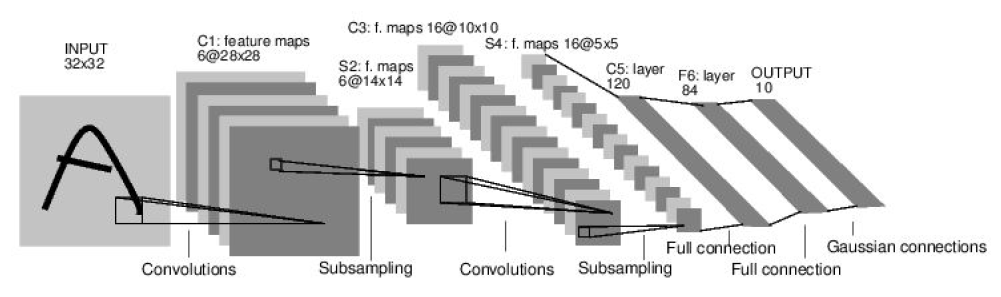
\includegraphics[width=10cm] {figures/LeNet-5.png}}        
	\caption{The Architecture of LeNet-5}      
	\label{LeNet-5}
\end{figure}
%\begin{figure}[htb]        
%	\center{\includegraphics[width=10cm] {AlexNet.png}}        
%	\caption{AlexNet}      
%\end{figure}

\begin{itemize}
	\item First of all, the input for LeNet-5 is digital picture with size $32 \times 32$ which every picture contains a number written by different writers. So, mathematically speaking, $x$ is a order 2 tensor with just one channel, with essential size $32 \times 32$, i.e $x \in \mathbb{R}^{ 1 \times 32 \times 32 }$.  And the out put is a 10-dimensional vector $\bm y = (y_0, \cdots, y_9)$ with $y_i$ equal to the probability for the number in $x$ is $i$. 
	
	\bigskip \hrule \bigskip
	\item Input: $x \in  \mathbb{R}^{ 1 \times 32 \times 32}$,  i.e 
	\begin{equation}
	\hat c_0 = 1, \quad \hat n_0 = 32.
	\end{equation}
	
	\item  $x \xrightarrow{\text{Convolution} ( \theta^0)} f^0$: 
	\begin{equation}
	\theta^0: \mathbb R^{1 \times 32 \times 32} \to \mathbb R^{6 \times 28 \times 28},
	\end{equation}
	ie.
	\begin{equation}
	c_0 = 6, \quad K^0 \in \mathbb R^{6 \times 1 \times 5 \times 5}, \quad b^0 \in \mathbb{R}^6.
	\end{equation}
	So we have the out put for the first layer as:
	\begin{equation}
	f^0 = \theta^0(x) \in \mathbb{R}^{6 \times 28 \times 28}.
	\end{equation}
	
	\bigskip \hrule \bigskip
	\item $f^0 \xrightarrow{\text{ReLU}(g) + \text{Pooling}(r^1)} y$: \\
	\begin{equation}
	g = \tau 
	\end{equation}
	and $r^1: \mathbb R^{6 \times 28 \times 28} \mapsto \mathbb R^{6 \times 14 \times 14} $ with max-pooling.
	So
	\begin{equation}
	y = g^1(f^0) \in \mathbb R^{6 \times 14 \times 14}.
	\end{equation}
	
	\item $y \xrightarrow{\text{Convolution}(\theta^1)} f^1$:
	\begin{equation}
	\theta^1: \mathbb R^{6 \times 14 \times 14} \to \mathbb R^{16 \times 10 \times 10},
	\end{equation}
	ie.
	\begin{equation}
	c_1 = 16, \quad K^1 \in \mathbb R^{16 \times 6 \times 5 \times 5}, \quad b^1 \in \mathbb{R}^{16}.
	\end{equation}
	So we have the out put for the first layer as:
	\begin{equation}
	f^1 = \theta^1(g^1(f^0)) \in \mathbb{R}^{16 \times 10 \times 10}.
	\end{equation}
	
	
	\bigskip \hrule \bigskip
	\item $f^1 \xrightarrow{\text{ReLU}(g) + \text{Pooling}(r^2)} y$: 
	\begin{equation}
	g = \tau 
	\end{equation}
	and $r^2: \mathbb R^{16 \times 10 \times 10} \mapsto \mathbb R^{16 \times 5 \times 5} $ with max-pooling.
	So
	\begin{equation}
	y = g2^(f^1) \in \mathbb R^{16 \times 5 \times 5}.
	\end{equation}
	
	\item {\bf Here we reshape $ y = g^2(f^1) \in \mathbb R^{16 \times 5 \times 5}$ as a vector in $\mathbb{R}^{400}$.}
	
	\item $y \xrightarrow{\text{affine map}(\theta^2) }f^3$: 
	\begin{equation}
	\theta^2: \mathbb R^{400} \to \mathbb R^{120},
	\end{equation}
	ie.
	with 
	\begin{equation}
	\theta^2(y) = W^2 y + b^2,
	\end{equation}
	here 
	\begin{equation}
	W^2 \in \mathbb{R}^{120\times 400}, \quad b^5 \in \mathbb{R}^{120}.
	\end{equation}
	So we have the out put for the fifth layer as:
	\begin{equation}
	f^2 = \theta^2(g^2(f^1)) \in \mathbb{R}^{120}.
	\end{equation}
	
	
	\bigskip \hrule \bigskip
	\item $f^2 \xrightarrow{\text{ReLU}(g) + \text{Pooling}(r^3)} y$: 
	\begin{equation}
	g = \tau 
	\end{equation}
	and $r^3 = id$.
	
	\item $y \xrightarrow{\text{affine map}(\theta^3)} f^3$: 
	\begin{equation}
	\theta^3: \mathbb R^{120} \to \mathbb R^{84},
	\end{equation}
	ie.
	with 
	\begin{equation}
	\theta^3(y) = W^3 y + b^3,
	\end{equation}
	here 
	\begin{equation}
	W^2 \in \mathbb{R}^{84\times 120}, \quad b^3 \in \mathbb{R}^{84}.
	\end{equation}
	So we have the out put for the fifth layer as:
	\begin{equation}
	f^3 = \theta^3(g^3(f^2)) \in \mathbb{R}^{84}.
	\end{equation}
	
	
	\bigskip \hrule \bigskip
	\item $f^3 \xrightarrow{\text{ReLU}(g) + \text{Pooling}(r^4)} y$: 
	\begin{equation}
	g = \tau 
	\end{equation}
	and $r^4 = id$.
	
	\item $y \xrightarrow{\text{affine map}(\theta^4)} f^4$: 
	\begin{equation}
	\theta^4: \mathbb R^{84} \to \mathbb R^{10},
	\end{equation}
	ie.
	with 
	\begin{equation}
	\theta^4(y) = W^4 y + b^4,
	\end{equation}
	here 
	\begin{equation}
	W^4 \in \mathbb{R}^{10\times 84}, \quad b^4 \in \mathbb{R}^{84}.
	\end{equation}
	So we have the out put for the fifth layer as:
	\begin{equation}
	f^4 = \theta^4(g^4(f^2)) \in \mathbb{R}^{10}.
	\end{equation}
	
	\bigskip \hrule \bigskip
	\item $f^4 \xrightarrow{\text{ReLU}(g) + \text{Pooling}(r^5)} y$: 
	\begin{equation}
	g = \tau 
	\end{equation}
	and $r^5 = id$.
	
	\item $y \xrightarrow{\text{affine map}(\theta^5)} f^5$: 
	\begin{equation}
	\theta^5: \mathbb R^{10} \to \mathbb R^{10},
	\end{equation}
	ie.
	with 
	\begin{equation}
	\theta^5(y) = W^5 y + b^4,
	\end{equation}
	here 
	\begin{equation}
	W^5 \in \mathbb{R}^{10\times 10}, \quad b^4 \in \mathbb{R}^{10}.
	\end{equation}
	So we have the out put for the fifth layer as:
	\begin{equation}
	f^5 = \theta^5(g^5(f^4)) \in \mathbb{R}^{10}.
	\end{equation}
\end{itemize}
\bigskip \hrule \bigskip

\begin{remark}
	The real LeNet-5 have two different structure with above $f^5$.
	\begin{enumerate}
		\item The structure for $\theta^1$ is a little special with they will fix some kernel as zeros such as:
		\begin{equation}
		K^1_{1,4:6} = 0
		\end{equation}
		and this structure can be found in the next figure:
		\begin{figure}[!htb]\label{LeNet-Channel}
			\center{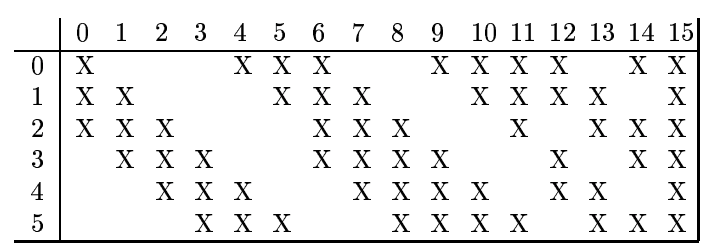
\includegraphics[width=10cm] {figures/LeNet-Channel.png}}        
			\caption{The ``0" Pattern for Channel Dimension of $K_{2,i}$}      
		\end{figure}
		
		\item The real out put is:
		\begin{equation}
		f^5 = f_{softmax}(g^5(f^4)).
		\end{equation}
	\end{enumerate}
	
	
\end{remark}



\subsection{An example of CNN model for Cifar-10}
We consider the data base CIFAR-10:
\begin{center}
	{\tt https://www.cs.toronto.edu/~kriz/cifar.html}.  
\end{center}

For Cifar-10, $\hat n_0 = n = 32$, $\hat c_0 = 3$ and $c = 10$. Here we construct a
model with $f(x; \Theta) = f^4$.

For simple, we set kernel size as $3 \times 3$ always, namely $k=1$.  
\begin{enumerate}
	\bigskip \hrule \bigskip  
	\item Here $\hat c_0 = 3$, we can set $c_0 = 32$, which means:
	\begin{equation}
	\theta^0 : \mathbb R^{2\times 32 \times 32} \to \mathbb R^{32 \times 32 \times32},
	\end{equation}
	with 
	\begin{equation}
	\theta^0(x) = K^0 \circledast x + {\rm{diag}(b^0) }\cdot \bm{1} \quad (\in
	\mathbb R^{32\times 32\times 32})
	\end{equation}
	where 
	$$
	K^0 \in R^{32 \times 3 \times 3 \times 3}, \quad b^0 \in \mathbb R^{32}
	$$
	$$
	\rm{diag}(b^0) 
	\in \mathbb R^{32\times 32}
	$$
	and 
	\begin{equation}
	(K^0 \circledast x)_p = \sum_{q = 1}^{\hat c_0 = 3} K^0_{p,q}\ast x \in \mathbb R^{28 \times 28}, \quad p = 1:c_0
	\end{equation}
	with 
	$$
	K^0_{p,q} \in \mathbb R^{3 \times 3} \quad p = 1:c_0, q = 1:3 .
	$$
	So we have:
	\begin{equation}
	f^0 = \theta^0( x)  \in \mathbb R^{32 \times 32 \times 32}.
	\end{equation}
	
	\bigskip \hrule \bigskip  
	\bigskip \hrule \bigskip  
	
	\item Then we apply activation function $g = \tau : \mathbb R^{32 \times 32 \times 32} \mapsto \mathbb R^{32 \times 32 \times 32} $ and keeping the size.  Here we just take $r^1 = id$.
	
	So we have, $\hat c_1 = c_0 = 32$, and $\hat n_1 = { n_0} = 32$, i.e
	\begin{equation}
	g^1: \mathbb R^{32 \times 32 \times 32} \mapsto \mathbb R^{32\times 32 \times 32}.
	\end{equation}
	
	\item Here $\hat c_1 = c_0 = 32$, we can still set $c_1 = 32$, so we have:
	\begin{equation}
	\theta^1 : \mathbb R^{32\times 32 \times 32} \to \mathbb R^{32 \times 32 \times32},
	\end{equation}
	with 
	\begin{equation}
	\theta^1(x) = K^1 \circledast x + {\rm{diag}(b^1)} \cdot \bm{1} \quad (\in
	\mathbb R^{32\times 32\times 32})
	\end{equation}
	where 
	$$
	K^1 \in R^{32 \times 32 \times 3 \times 3}, \quad b^1 \in \mathbb R^{32}
	$$
	$$
	\rm{diag}(b^1) 
	\in \mathbb R^{32\times 32}
	$$
	and 
	\begin{equation}
	(K^1 \circledast x)_p = \sum_{q = 1}^{\hat c_1 = 32} K^1_{p,q}\ast x \in \mathbb R^{28 \times 28}, \quad p = 1:32
	\end{equation}
	with 
	$$
	K^1_{p,q} \in \mathbb R^{3 \times 3} \quad p = 1: c_1, ~  q = 1: \hat c_1 .
	$$
	So we have 
	\begin{equation}
	f^1 = \theta^1( g^1(f^0))  \in \mathbb R^{32 \times 32 \times 32}.
	\end{equation}
	
	\bigskip \hrule \bigskip  
	\bigskip \hrule \bigskip  
	\item For this layer, we also apply $g = \tau$, however we apply pooling function $r^2: \mathbb R^{32 \times 32 \times 32} \mapsto \mathbb R^{32 \times 16 \times16} $ with fix-position pooling:
	$$
	r^1(X)_{i,j} = X_{2i, 2j}, \quad  i, j = 1:14.
	$$ 
	or max pooling:
	$$
	r^1(X)_{i,j} = \max_{-1 \le k,l \le 0}X_{2i+k, 2j+l}, \quad i , j = 1:14.
	$$
	Here, we take max-pooling. 
	
	So we have, $\hat c_2 = c_1 = 32$, but $\hat n_2 = \frac{ n_1}{2} = 16$, i.e
	\begin{equation}
	g^2: \mathbb R^{32 \times 32 \times 32} \mapsto \mathbb R^{32\times 16 \times 16}.
	\end{equation}
	
	\item Here $\hat c_2 = 32$ and $\hat n_2 = 14$, we may also set $c_2 = 64$, so we have parameters 
	$$
	K^2 \in \mathbb R^{64 \times 32 \times 3 \times 3},\quad b^2 \in \mathbb R^{64}
	$$
	then we have 
	\begin{equation}
	\theta^2: \mathbb R^{32 \times 16 \times 16} \mapsto \mathbb R^{64 \times 16 \times 16}.
	\end{equation}
	Note $y = g^2 (f^1)$ so we have,
	\begin{equation}
	\theta^2(y) = K^2 \circledast y + {\rm{diag}(b^2)} \cdot \bm{1}, 
	\end{equation}
	and 
	\begin{equation}
	(K^2 \circledast y)_p = \sum_{q = 1}^{\hat c_2 = 32} K^2_{p,q} \ast y_q \in \mathbb R^{14 \times 14}, \quad p = 1:64
	\end{equation}
	with 
	$$
	K^2_{p,q} \in \mathbb R^{3 \times 3},\quad p = 1:64, q = 1:32.
	$$
	So we have the out put for the second layer as:
	\begin{equation}
	f^2 = \theta^2(g^2(f^1)) \in \mathbb R^{64 \times 16 \times 16}.
	\end{equation}
	
	
	
	\bigskip \hrule \bigskip  
	\bigskip \hrule \bigskip
	\item For this layer, we also apply $g = \tau$, then apply pooling function $r^3: \mathbb R^{64 \times 16\times 16} \mapsto \mathbb R^{64 \times 8 \times 8} $ with $r^3$ as max-pooling.
	
	So we have, $\hat c_2 = c_1 = 64$, but $\hat n_3 =  \frac{n_2}{2} = 7$, i.e
	\begin{equation}
	g^3: \mathbb R^{64 \times 16\times 16} \mapsto \mathbb R^{64 \times 8 \times 8}.
	\end{equation}
	
	\item {\bf Here we reshape $g^3(f^2) \in \mathbb R^{64 \times 8 \times 8}$ as a vector in $\mathbb{R}^{4096}$.}
	
	\item Let $y = \rm{Vec}(g^3(f^3))$, for this layer, we apply the fully connected(general DNN model) for $y$ with:
	\begin{equation}
	\theta^3: \mathbb{R}^{4096} \to \mathbb R^{120},
	\end{equation}
	with 
	\begin{equation}
	\theta^3(y) = W^3 y + b^3,
	\end{equation}
	here 
	\begin{equation}
	W^3 \in \mathbb{R}^{120\times 4096}, \quad b^4 \in \mathbb{R}^{120}.
	\end{equation}
	
	So we have the out put for the fifth layer as:
	\begin{equation}
	f^3 = \theta^3(g^3(f^2)) \in \mathbb{R}^{120}.
	\end{equation}
	
	\bigskip \hrule \bigskip  
	\bigskip \hrule \bigskip
	\item For this layer, we also apply $g = \tau$, and $r^4 = id$, so $g^{4}(f^3) \in \mathbb{R}^{120}$.
	
	\item Then let's set $n_4 = c =  10$, and let $y = g^4(f^3)$  i.e 
	\begin{equation}
	\theta^4: \mathbb{R}^{120} \to \mathbb R^{10},
	\end{equation}
	with 
	\begin{equation}
	\theta^4(y) = W^4 y + b^4,
	\end{equation}
	here 
	\begin{equation}
	W^4 \in \mathbb{R}^{10\times 120}, \quad b^4 \in \mathbb{R}^{10}.
	\end{equation}
	So we have the out put for the fifth layer as:
	\begin{equation}
	f^4 = \theta^4(g^4(f^3)) \in \mathbb{R}^{10}.
	\end{equation}
\end{enumerate}


\section{New notation for general DNN}
Motivated by the ResNet model and the newly changed version for ResNet model, we may construct those next neural network notation for better understand about all kinds of DNN and CNN models.


Here we want to reconstruct our notation for general DNN model with we proposed ``level" not ``layer" with we can construct some fake layers between two different levels. For general DNN model, the notation is totally same with we just replace layers as levels. But when we consider about the CNN model, we emphasize that the level index increase only after the essential dimension for the data changes.

\subsection{Stride and Pooling}
Here we first reanalysis this two important operator in general CNN model, which change the essential dimension for data. Let us recall the definition of those two operator:
\begin{definition}{Stride}
	\begin{equation}
	S(x_1, \cdots, x_p) = x_q, \quad  1 \le q \le p.
	\end{equation}
\end{definition}

\begin{definition}{Pooling}
\begin{equation}
P(x_1, \cdots, x_p) = r(x_1, \cdots, x_p),
\end{equation}
\end{definition}
where $r$ is a nonlinear or linear restriction function.

Let us recall where those two operation is used. In general, stride is used after the general convolution and the pooling is used after he nonlinear activation function.  Here we can also note pooling as before the convolution, so we can note the stride or pooling with general convolution together as:
\begin{equation}\label{stride-pooling}
\tilde \theta = \theta \circ S, \quad \text{or} \quad \tilde \theta = P\circ \theta.
\end{equation}
\begin{remark}
	Here we can take $P = id$ such that $\tilde \theta$ can also work as the general convolution operator.
\end{remark}

\subsection{New Notation with Level Index}

So we have the next expression:
\begin{equation}\label{new-dnn}
\begin{cases}
	f^j &= \tilde \theta^j\circ \mathcal{H}^j_{l_j} \circ g(f^{j-1}), \\
	f^0 &= \tilde \theta^0(x).
\end{cases}
\end{equation}
Here we note that, if $l_j = 0$ then $\mathcal{H}^j_{l_j} = id$.

Here $\mathcal{H}^j_{l_j}$ works like the classical DNN model as people often used version for DNN:
\begin{equation}
	\mathcal{H}_{l_j}^j (x) = g \circ \theta^{j,{l_j}}  \cdots g \circ \theta^{j,{l_1}} (x),
\end{equation}
here we emphasize that $\theta$ are all general convolutions.



\section{New notation on the same level $\ell$}
This is analogous to the smoothings carried on each level.  But this
time, it is a sequence of nonlinear operations. 

Input $y$, and output $z$:
$$
z=H^\ell(y)
$$
Based on the approximation theory, let us construct a basic nonlinear block for our net work as:
\begin{equation}\label{eq1-basic}
F_k(x) = \xi^k \circ g \circ \eta^k(x),
\end{equation}
\section{From level $\ell$ to $\ell+1$: restriction}

\begin{enumerate}
\item Input:  $f^\ell$
\item output:  $f^{\ell+1}_0 = R_{\ell}^{\ell+1}f^{\ell}$
\end{enumerate}

Here 
$$
 R_{\ell}^{\ell+1}: \mathbb R^{n_\ell}\mapsto \mathbb R^{n_{\ell+1}}
$$
can be given by either
\begin{enumerate}
\item pooling, or
\item convolution with stride.
\end{enumerate}

\section{Plain nets}

\subsection{Same level}
$$
y_1=F_1(y)
$$
$$
y_{k+1}=F_k(y_{k})
$$
$$
z=y_{m_\ell}
$$
We define
$$
H^\ell(y)=y_{m_\ell}.
$$

We note that
$$
F_{k+1}(F_{k}(y_k))
=(\xi^{k+1} \circ g \circ \eta^{k+1})[(\xi^k \circ g \circ \eta^k)(y_k)]
=(\xi^{k+1} \circ g \circ (\eta^{k+1}\xi^k)\circ g \circ\eta^k)(y_k)
$$
In the most general DNN, we can make the following combination:
$$
\eta^{k+1}\xi^k=\tilde \eta^k.
$$
But in the context CNN, we may not simply do this combination?

\subsection{Multilevel}
$$
f^{\ell+1}=H^{\ell+1}\circ (R_{\ell}^{\ell+1}f^\ell)
$$

\section{ResNet in this Notation}
\subsection{Same level}
$$
y_1=F_1(y)
$$
$$
y_{k+1}=y_k+  F_k(y_{k})
\quad k=1,\ldots m_\ell-1.
$$

\bigskip
\hrule  
Here we note that, if the dimension is suitable we may have:
\begin{align}
F_k(x) &= \xi \circ g \circ  \eta (x) = ( \tilde \xi - \hat \xi) \circ g \circ \eta (x) \\
&= \tilde \xi \circ g \circ \eta (x) - \hat \xi \circ g \circ \eta(x) \\
&=  \tilde \xi \circ g \circ \eta (x)  - x .
\end{align}
\hrule 
\bigskip

\hrule 
\bigskip 
In the linear case, let $y$ be a given vector, if we apply a smoother,
we can have the following
$$
y_{k+1}=(I-\omega A) y_k
=y_k-\omega A y_k
$$
In this case, we can view
$$
F_k=-\omega A.
$$
\bigskip 
\hrule 
\bigskip

In the end,  the output is
$$
z=y_{m_\ell}=y_1+\sum_{j=2}^{m_\ell} F_j(y_j)
$$
and
$$
f^\ell=z.
$$
\subsection{Multilevel}
$$
f^{\ell+1}=H^{\ell+1}\circ (R_{\ell}^{\ell+1}f^\ell)
$$

In the original work of He Kaiming:
$$
f^{\ell+1}=H^{\ell+1}\circ (R_{\ell}^{\ell+1}f^\ell+P^\ell y_{m_\ell-1}^\ell)
$$
Notice that
$$
R_{\ell}^{\ell+1}f^\ell+P^\ell y_{m_\ell-1}^\ell=
R_{\ell}^{\ell+1}[F_{m_\ell-1}(y_{m_\ell-1}^\ell)+ y_{m_\ell-1}^\ell]+P^\ell y_{m_\ell-1}^\ell=
$$


\section{Multiple coarse spaces: general CNN}
This notation originally was contained in $\theta$ in the original
notations. But now, for better understand we are going to investigate
the structure for general $\theta$ in CNN.

Let us focus on level $\ell$, the output of level $\ell$ consists of
$c_\ell$ images:
\begin{equation}
  \label{Xl}
X^\ell_{j}:  j=1:c^\ell.  
\end{equation}
For $\ell=0$, we have
$$
c_0=
\left\{
  \begin{array}{lr}
1 & \mbox{ grey}\\    
3 & \mbox{color}
  \end{array}
\right.
$$
$$
c^{\ell+1}_i: i=0,1,\ldots m_{\ell+1}
$$
with 
$$
c^{\ell+1}_0=c_\ell.
$$

Assume that $c^{\ell+1}_{i}$ is known.   That we have the following
number of images:
$$
X^{\ell+1,i}_{j}:\quad j=1:c^{\ell+1}_i
$$
We need to define
$$
X^{\ell+1,i+1}_{j}:\quad j=1:c^{\ell+1}_{i+1}.
$$

$$
X^{\ell+1,i+1}_{j}=
g\bigg(
\sum_{k =1}^{c^{\ell+1}_{i}}X_k^{\ell, i}\ast K^i_{j,k}
\bigg) 
$$
The final outcome is
$$
X^{\ell+1}_{j}\equiv 
X^{\ell+1,m_{\ell+1}}_{j}= 
g\bigg(
\sum_{k =1}^{c^{\ell+1}_{m_{\ell+1}-1}}X_k^{\ell, m_{\ell+1}-1}\ast K^{m_{\ell+1}-1}_{j,k}
\bigg),\quad  j=1:c^{\ell+1}_{m_{\ell+1}}.
$$

For general CNN model to deal with the single channel image $X$, they first use some different $K_i$ to do smooth for $X$ in and get multiple smoothed image as $K_i \ast x$ for $i = 1:c_0$ and do activation function for those multiple smoothed image and get $g(K^0_i \ast X)$, like:
\bigskip
\hrule
Input: $X$, output $\tilde Y_i$:
\begin{equation}
\tilde Y_i = g(K^0_i \ast X), \quad i = 1:c_0
\end{equation}
\hrule
\bigskip
Then the next operation is the most different and interesting operations in CNN which is different from the general pure convolution(smoother). Now we suppose to get just one channel image first for $Y_i$, they use
\bigskip
\hrule
Input: $\tilde Y_i$, output $Z$:
\begin{equation}
Z = \sum_{i=1}^{c_0} \tilde Y_i \ast K^1_i
\end{equation}
\hrule


\newpage
\subsection{Xu idea}
Here we begin with a single channel image as $X \in \mathbb{R}^{n\times n}$, now we state that Prof. Xu's idea can be implement by the general CNN convolution operation.  
\bigskip
\hrule
Input: $X$, output $Y$:
\begin{equation}
Y = \sum_{i=1}^c a_i g(K_i \ast X),
\end{equation}
\hrule
\bigskip

So, as for now, if we take $K^1_i = a_i I$, then we have $Z = Y$ as Prof. Xu's idea. 

Here we can note that, in $Y$ level we have $\tilde Y_i$ with $i=1:c$ multiple smoothed image or we say you have detected $c$ features from the $X$ level, so in $Z$ level we may also construct $i = 1:c_1$  multiple space to save those $c_1$ features, so what we do generally in CNN is:
\bigskip
\hrule
Input: $\tilde Y_i$, output $Z_j$:
\begin{equation}
Z_j = \sum_{i=1}^{c_0} \tilde Y_i \ast K^1_{i,j}, \quad j = 1:c_1
\end{equation}
\hrule
\bigskip

And after that, you can do the similar things like from $Y$ level to $Z$ level with multiple space operation. 

\section{DenseNet in this notation}
\subsection{same level}

$$
H^{j}(x) = \theta^j \circ g \circ BN
$$
$$
y_{k+1}= H^{k}([y_k, y_{k-1},\cdots, y_0]).
\quad k=1,\ldots m_\ell-1.
$$


\newpage
\section{some other observations}
Now let us think about that we have $X = (X_1, X_2, X_3)$ with $X_i \in \mathbb{R}^{n\times n}$. That's to say now we have $3$ coarse space first, now we want to do some convolution or we say as smoother in AMG. Here we 

Prof. Xu's idea is to say that, we need to keep the original ``channel" parallel i.e we just need three kernels like 
\begin{align}
	K_0 = \begin{pmatrix}
		K^1 \\ K^2 \\ K^3
	\end{pmatrix}.
\end{align} So we get:
\begin{equation}
X \to X\tilde{\ast} K_0 = (X_1 \ast K^1, X_2\ast K^2, X_3 \ast T^3),
\end{equation}
and then we apply the active function $a$ to $(X_1 \ast K^1, X_2\ast K^2, X_3 \ast T^3)$ element by element. And then use 
\begin{align}
	X^{new} = (a(X_1 \ast K^1), a(X_2\ast K^2), a(X_3 \ast T^3))
\end{align} as the next input for the CNN network.

Now we want to show that the traditional method with more kernels can reproduce the $X^{new}$ in Prof. Xu's case.

Here we set we have some more kernels like 
\begin{align}
	K = 
	\begin{pmatrix}
		K_1^1 & \cdots & K_1^N \\
		K_2^1 & \cdots & K_2^N \\
		K_3^1 & \cdots & K_3^N 
	\end{pmatrix},
\end{align} with $K_i^j \in \mathbb{R}^{3\times3}$.

What we have at most are:
\begin{equation}
\tilde{X} = X\tilde{\ast} K =  \begin{pmatrix}
X_1 \ast K_1^1 & \cdots & X_1\ast K_1^N \\
X_2 \ast K_2^1 & \cdots & X_2\ast K_2^N \\
X_3 \ast K_3^1 & \cdots & X_3\ast K_3^N 
\end{pmatrix}
\end{equation}

{\bf Here in fact we can have a simple question: why we don't just put $a(\tilde{X})$ as the next input for the next layer of CNN? Maybe this dimension is to large?}

Traditional method for convolution with channel is to say we need to compress the original ``channel" dimension by take 
\begin{equation}
\tilde{X}  \to ( \sum_{j=1:3} X_j\ast K_{j}^1, \cdots, \sum_{j=1:3} X_j\ast K_{j}^N),
\end{equation} 
and then apply the active function $a$ getting:
\begin{equation}
(a( \sum_{j=1:3} X_j\ast K_{j}^1), \cdots, a(\sum_{j=1:3} X_j\ast K_{j}^N)).
\end{equation}

So we can see that, if we take $ N = 3$ then we can reproduce the 
$T^{new} = (a(X_1 \ast K^1), a(X_2\ast K^2), a(X_3 \ast T^3))$ from $(a( \sum_{j=1:3} X_j\ast K_{j}^1), \cdots, a(\sum_{j=1:3} X_j\ast K_{j}^N))$ by just take
\begin{align}
	K^i = \sum_{j=1:3} K_j^i, \quad \forall i = 1:3.
\end{align}

\begin{remark}
	Here we can take Prof. Xu's idea and the traditional convolution as consistent by means that because the dimension for $a(\tilde{X})$ is too large({\bf In fact, we like redundancy some times, why we just use this directly?}), we need some ways to compress $\tilde{X}$ first and then apply active function $a$. The simplest next two ways is:
	\begin{itemize}
		\item Compress(sum) $\tilde{X}$ in row. This leads to Prof. Xu's idea keeping the ``channel" number as 3.
		\item Compress(sum) $\tilde{X}$ in column. This leads to traditional idea changing the ``channel" into $N$.
	\end{itemize}
	
	{\bf Another questions is how to compress this $\tilde{X}$ ``better"?  What dose better means?}
	
\end{remark}


%\chapter{Connection of 1D CNN and DNN}
\section{1D CNN as DNN}
First let us consider a CNN model for 1D date i.e. $x \in \mathbb{R}^d$ as:
$$
(v\ast x)_i = \sum_{k=1}^d w_{i-k+1}x_k, \quad \forall i = 1:d+s,
$$
with 
$$
v \in \mathbb{R}^s.
$$
This lead to a $(d+s)\times d$ Toeplitz type convolutional matrix $T^v$ defined by
$$
(T^v)_{i,j} = v_{i-k+1}, \quad i=1:d+s, k = 1:d.
$$

This kind of convolution can be think as ``padding" for not only data but also kernel.
So, this will lead to an increasing of dimensional for output.

Here, we consider ``restriction-activation'' functions as only activation functions,
and alway only have one channel, so we have the CNN model  as:
\begin{equation}\label{CNN_iteration_vector}
f^j(x,\Theta^j) = v^j \ast( g \circ f^{j-1})(x,\Theta^{j-1}) + b^j \in \mathbb{R}^{d + (j+1) \times s }
\end{equation}
where
\begin{equation}
\Theta^j=(\Theta^{j-1},v^j), \quad \Theta^0=(v^0, b^0) 
\end{equation}
with 
\begin{equation}
f^0(x)=v^0 \ast x + b^0,
\end{equation}
and 
\begin{equation}\label{CNN_finallayer}
f(x; \Theta) = f^J.
\end{equation}

Then we say that, use CNN to approximate function is in the class:
$$
\mathcal{H} = \{ \sum_{i= 1}^{d_J} c_i f^J_i(x): c \in \mathbb{R}^{d_J}\},
$$
here $d_j = d + (j+1)\times s$, is the dimension of $f^j$. 

Now let us consider, we have a one hidden layer DNN model as:
$$
f_{DNN} = \sum_{i=1}^m \alpha_k g( w_i x + b_k),
$$ 
then we can construct 
$$
W = [w_1, w_2, \cdots, w_m], \in \mathbb{R}^{1\times(md)},
$$
then we have the next decomposition as
$$
W\ast x = w^{\hat J-1} \cdots w^1\ast w^0 \ast x,
$$
for 
$$
\hat J \le \frac{md}{s-1} +2.
$$

Now, we have a new CNN model as:
\begin{equation}\label{CNN_iteration_vector}
f^j(x,\Theta^j) = v^j \ast \circ f^{j-1}(x,\Theta^{j-1}) + b^j \in \mathbb{R}^{d + (j+1) \times s }
\end{equation}
and 
$$
f^J(x,\Theta^J) = w^J \ast ( g\circ f^{J-1})(x,\Theta^{J-1}) \in \mathbb{R}^{d + (J+1) \times s },
$$
where
\begin{equation}
\Theta^j=(\Theta^{j-1},v^j), \quad \Theta^0=(v^0, b^0) 
\end{equation}
with 
\begin{equation}
f^0(x)=v^0 \ast x + b^0,
\end{equation}
and 
\begin{equation}\label{CNN_finallayer}
f(x; \Theta) = f^J.
\end{equation}
Then we can choose $w^j$ as delta i.e identity map for $j \ge \hat J$, and for the last model
$$
f_{CNN} = \sum_{i= 1}^{d_J} c_i f^J_i(x),
$$
we can have
$$
f_{CNN} = f_{DNN},
$$
by choosing $c$ coefficients and $b^j$ carefully. [As homework.]
So all approximation properties for one hidden layer DNN can be reconstructed for CNN.

\begin{theorem}
	For one dimensional kernel, we have the decomposition as
	$$
	W\ast x = w^{\hat J-1} \cdots w^1\ast w^0 \ast x.
	$$
\end{theorem}
\begin{proof}
	This proof is in the literature of Daubechies 1992.  Let us define the symbol $\tilde w$ as a polynomial on $\mathbb{C}$ by 
	$$
	\tilde w (z) = \sum_{i=1}^s w_{i}z^{i-1}.
	$$
	The most important result is that
	$$
	\tilde w(z) \tilde v(z) = \widetilde{(w\ast v)}(z).
	$$
	Then we know that for any polynomial with real coefficients it can be decomposed as 
	$$
	\tilde W(z) = W_M \Pi_{k=1}^K\{z^2 - 2\alpha_kz + (\alpha_k^2 + \beta_k^2)\} \Pi_{2K+1}^{M-1}(z - \alpha_k).
	$$
	This means that, for $s \le 2$, we can combine the above decomposition with every $\tilde w^j(z)$ is a $s-1$-degree of polynomial ans
	$$
	\tilde W(z) = \tilde w^{\hat J-1}(z)\cdots \tilde w^{1}(z)\tilde w^{0}(z).
	$$
\end{proof}

